\documentclass[12pt,oneside,nocenter,noupper,bold]{teseir}
%\documentstyle[12pt,a4,oneside,nocenter,noupper,bold,epsf,multicol,graphicx,here]{teseir}
%\graphicspath{.}
\usepackage{graphicx}
\usepackage{bm}
\usepackage[brazil]{babel}% separa silaba
\usepackage{graphicx}% insercao de figuras
\usepackage{t1enc}% reconhece acentuacao
\usepackage{amsmath}%caracteres matematicos
\usepackage{physics}
\usepackage{tikz-feynman}
\usepackage{natbib}
\bibliographystyle{plain}

\oddsidemargin 0pt
\evensidemargin 6pt
\textwidth 460pt
\textheight 670pt
  \newcounter{bean}
  \setlength{\unitlength}{1.5cm}
\renewcommand{\baselinestretch}{1.5}

%\textwidth 16 cm
%\textheight 25 cm
\topmargin -.5 cm
%\oddsidemargin -.1cm

% Para separar silabas em portugues:
\language=1

%%%%Para meter um header nas paginas:
\pagestyle{headings}

%%% aqui os arquivos definitivos
\includeonly{c,pagbranco,cap1,cap2,cap3,cap4,cap5, ref3}

\begin{document}

\hyphenation{re-pre-sen-ta-da}
\hyphenation{des-pre-za-das}
\hyphenation{va-lo-res}
\hyphenation{i-ma-gi-ná-ria}

\pagenumbering{arabic}
\begin{titlepage}
\begin{center}\Large
{UNIVERSIDADE FEDERAL DO RIO GRANDE DO SUL \\
INSTITUTO DE FÍSICA}
\end{center}
\vfill
\begin{center}\Large
\renewcommand{\thefootnote}{\fnsymbol{footnote}}
\setcounter{footnote}{1}
{\bf Fotoprodução exclusiva de mésons vetoriais  pesados $J/\Psi$ em colisões Pb-Pb em NLO}%
\end{center}

\bigskip

\begin{center}
\Large
Eliton Trindade Gomes
\end{center}
\bigskip

\vfill
\hfill
\begin{minipage}[b]{0.6\textwidth}
Disserta\c{c}\~ao  realizada sob a orienta\c{c}\~ao da Professora Dra.
Maria Beatriz Gay Leony Ducati e apresentada ao
Instituto de F\'{\i}sica da UFRGS, em preenchimento
parcial dos requisitos para a obten\c{c}\~ao do t\'{\i}tulo
de Mestre em F\'{\i}sica.
\end{minipage}
\setcounter{footnote}{0}
\renewcommand{\thefootnote}{\arabic{footnote}}
\vfill
\begin{center}
{Porto Alegre \\ 2024}
\end{center}
\end{titlepage}

%\include{pagbranco}
%\include{dedica}
%\include{dedica1}
%\include{pagbranco}
%\include{agrad}
%\include{pagbranco}
%\include{abstract}
\tableofcontents
%\include{pagbranco}
\listoffigures
\newpage
\chapter{Espalhamento Compton Profundamente Virtual~(DVCS)}
\label{cap:cap1}
\section{Introdução}
Uma área importante da física de partículas é a investigação da estrutura interna dos hádrons; isso é essencial para a compreensão dos componentes essenciais da matéria. O espalhamento elástico e inelástico são apenas alguns dos vários métodos experimentais e teóricos utilizados para abordar esta investigação.
Os processos elásticos fornecem informações cruciais sobre os fatores de forma do núcleo, permitindo uma compreensão detalhada da distribuição de carga e da estrutura interna dos hádrons. Por outro lado, os processos inelásticos, como a Espalhamento inelástico profundo (DIS), oferecem uma visão mais profunda das Funções de Distribuição de Pártons (PDFs), que descrevem as probabilidades de encontrar pártons com uma determinada fração do momento do hádron.

Apesar de serem complementares, ambos os métodos têm suas próprias limitações. Os fatores de forma não revelam informações diretas sobre a distribuição espacial dos pártons e as PDFs não fornecem uma compreensão direta do momento dos constituintes hadrônicos. Para superar tais restrições e unificar os conceitos de distribuições de momento e espaciais, as Distribuições de Pártons Generalizadas (GPDs) têm sido ferramenta essencial neste processo.

As GPDs  desempenham um papel importante em processos exclusivos de DIS, como o Espalhamento Compton Profundamente Virtual (DVCS),  Fotoprodução Exclusiva de Mésons Vetoriais Pesados (HVMP),  onde a correlação entre a distribuição espacial e a fração de momento dos pártons dentro do hádron pode ser estudada em detalhes. O DVCS é um processo fundamental que oferece uma visão única da estrutura interna dos hádrons, permitindo uma exploração mais profunda das propriedades das GPDs e uma compreensão mais completa da natureza dos constituintes hadrônicos.

Neste capítulo, é apresentado conceitos fundamentais do estudo de estrutura interna dos hádrons. Para isso, abordamos os processos de espalhamento elástico $ep \rightarrow e' p'$ e espalhamento  inelástico profundo $eN \rightarrow e' X$, onde são apresentados os fatores de forma e funções de distribuição de pártons, respectivamente.   Posteriormente, apresentamos as GPDs que são base do estudo  de foto-produção de mésons vetoriais realizada neste trabalho,  a partir da abordagem do DVCS que representa o seguinte processo:
\begin{equation}
    p + e \rightarrow p' + e' + \gamma
\end{equation}

\section{Distribuição e fatores de forma}
\subsection{Fatores de forma - espalhamento elástico}
\paragraph{}
O estudo do espalhamento elástico de elétron-próton ($e + p \rightarrow e' + p'$, ver  Fig. \ref{fig:elast-ep}) é fundamental para investigar a estrutura interna dos hádrons. Esse processo fornece informações cruciais sobre a distribuição de carga e magnetismo dentro do próton, revelando detalhes sobre a organização espacial de seus constituintes.
\begin{figure}[!ht]
    \centering
    \begin{tikzpicture}
        \begin{feynman}
            \vertex (a);
            \vertex [right=2cm of a] (b);
            \vertex[above right=1cm and 2cm  of b](e);
            \vertex [below=2.5cm of a] (c);
            \vertex [right=2cm of c] (d);
            \vertex[below right=1cm and 2cm  of d](f);
            \diagram*{
            (a) -- [fermion, edge label=$k$] (b),
            (c) -- [double,double distance=0.25ex,thick,with arrow=0.5,edge label=$p$] (d),
            (b) -- [photon, edge label=$\gamma^*(q)$] (d),
            (b) -- [fermion, edge label=$k'$](e),
            (d) -- [double,double distance=0.25ex,thick,with arrow=0.5, edge label=$p'$](f)
            };
            \draw[fill=black] (a) circle (0.1cm) node[left] {$e^-$};
            \draw[fill=black] (c) circle (0.1cm) node[left] {$p^+$};
            \draw[fill=black] (e) circle (0.1cm) node[above right]{$e^-$};
            \draw[fill=black] (f) circle (0.1cm) node[below right]{$p^+$};
        \end{feynman}
    \end{tikzpicture}
    \caption{Diagrama de Feynman para colisão elástica elétron-próton}
    \label{fig:elast-ep}
\end{figure}

A análise desse espalhamento é comumente realizada por meio dos chamados fatores de forma, que descrevem a extensão espacial dos núcleos e relacionam a seção de choque do processo com uma carga pontual. Modelos como  o espalhamento de Rutherford, desenvolvida em 1911~\cite{rutherford} para partículas alfa espalhadas em folhas de ouro, foram fundamentais inicialmente para entender esse processo em casos não relativístico. Para os casos relativísticos, o Espalhamento de Mott  é mais apropriado.

A matriz de amplitude para esse processo é dada por:
\begin{equation}
    \mathcal{M} = \qty[\mu (k')\gamma^\mu u(k)] \frac{e^2}{q^2} \qty[\overline{u}(p')\Gamma_\mu u(p)],
    \label{eq:matrizelastica}
\end{equation}
onde $q=(k-k')$ é $ie\Gamma_\mu$ é o fator de vértice do próton, no qual,
\begin{equation}
    \Gamma_\mu = \qty[F_1(q^2)\gamma^\mu + \frac{F_2(q^2)}{2M}i \sigma^{\mu \alpha}q_\alpha ].
\end{equation}
Aqui, $\sigma^{\mu\nu} = (i/2)[\gamma^\mu, \gamma^\nu]$ e $F_1(q^2)$, $F_2(q^2)$ são os fatores de forma de Dirac e Pauli,~respectivamente. Esses fatores de forma são independentes e no limite  $q^2\rightarrow 0$ são $F_1(0)=F_2(0)=1$.

A partir da matriz de Amplitude \eqref{eq:matrizelastica},  obtemos que a seção de choque para  espalhamento elástico de elétrons em prótons no referencial do laboratório, com o próton inicialmente em repouso é dada por:
\begin{eqnarray}
    \qty(\dv{\sigma}{\Omega})_{(lab)}&=&\frac{\alpha^2 }{4 E^2 sen^4 (\theta/2)} \frac{1}{1+(2E/M)sin^2(\theta/2)}\times\nonumber\\&&\qty[\qty(F_1^2(q^2) - \frac{q^2 \kappa^2F_2(q^2)}{4M^2})cos^2\qty(\theta/2) - \frac{q^2}{2M^2}\qty(F_1(q^2) + \kappa F_2(q^2))^2 sen^2\qty(\theta/2)]
    \nonumber\\\nonumber\\
    &=&\qty(\dv{\sigma}{\Omega})_{(Mott)}\qty[1+\frac{2E}{M}sen^2 \qty(\frac{\theta}{2})]^{-1}\times\nonumber\\&&\qty[\qty(F_1^2(q^2) - \frac{q^2 F_2(q^2)}{4M^2}) - \frac{q^2}{2M^2}\qty(F_1(q^2) + F_2(q^2))^2 tang^2\qty(\theta/2)],
\end{eqnarray}
onde a massa do elétron $m_e$ é desprezada. Essa equação pode ser reescrita a partir fatores de forma $G_E(q^2)$ e $G_M(q^2)$, que representam a distribuição de carga e momento magnético, respectivamente. Esses fatores de forma se relacionam aos fatores de forma de Dirac e Pauli partir das equações:
\begin{align}
    G_E(q^2) & = F_1(q^2) - \frac{q^2}{4M^2}F_2(q^2), \\
    G_M(q^2) & = F_1(q^2) + F_2(q^2).
\end{align}
Portanto, temos a equação geralmente utilizada para descrever o espalhamento elástico de elétrons em prótons,  fórmula de Rosenbluth:
\begin{equation}
    \frac{d\sigma}{d\Omega} = \frac{\alpha^2}{4E^2}\sin^4\left(\frac{\theta}{2}\right)\frac{E'}{E}\left(G_E^2(q^2) + \tau G_M^2(q^2)\frac{(1 + \tau)}{\cos^2(\theta/2)} + 2\tau G_M^2(q^2)\sin^2(\theta/2)\right),
    \label{eq:rosenbluth}
\end{equation}
onde $\tau = -q^2/4M^2$. A equação \eqref{eq:rosenbluth} oferece uma descrição detalhada da distribuição angular da seção transversal do espalhamento, incorporando os fatores de forma $G_E(q^2)$ e $G_M(q^2)$ que caracterizam a estrutura interna do próton. Essa equação nos permite compreender em detalhes o espalhamento elástico de elétrons em prótons, considerando os fatores de forma que refletem a distribuição de carga e momento magnético do próton.

\subsection{Espalhamento Inelástico Profundo: Distribuições de Pártons}


Consideremos o processo inclusivo \( e + N \rightarrow e + X \), no qual um elétron é espalhado por um núcleon, resultando em uma combinação de partículas finais (\( X \)). Esses processos fornecem informações sobre a distribuição do momento dos pártons dentro do núcleon.
\begin{figure}[!ht]
    \centering
    \begin{tikzpicture}
        \begin{feynman}
            \vertex (a){\(e^-\)};
            \vertex [below right= 1cm and 2cm of a] (b);
            \vertex [above right=1cm and 2cm of b] (c);
            \vertex [below right=1cm  and 1cm of b, blob] (d){};
            \vertex [below left=1cm and 2cm of d] (e){N};
            \vertex[below right= 0.3cm and 1.5cm of d ](f);
            \vertex[right= 1.8cm of d ](g){x};
            \vertex[above right= 0.3cm and 1.5cm of d ](h);

            \diagram* {
            (a) -- [fermion, edge label=\(k\)] (b),
            (b) -- [fermion, edge label=\(k'\)] (c),
            (e) -- [double,double distance=0.25ex,thick,with arrow=0.5, , edge label=\(p\)] (d),
            (b) -- [boson, edge label'=\(\gamma^*(q)\) ] (d),
            (d) -- [fermion](f),
            (d) -- [fermion](g),
            (d) -- [fermion](h),
            };
        \end{feynman}
    \end{tikzpicture}
    \caption{Espalhamento inelástico profundo de um elétron em um nucleon }
    \label{fig:dis}
\end{figure}

No espalhamento inelástico profundo (DIS), representado na Fig.~\ref{fig:dis}, apenas o elétron espalhado é detectado, portanto, há alguma energia do estado inicial que não é detectada no estado final. Neste processo um elétron inicial \( e(k) \) interage com o núcleon $N(p)$ em seu estado inicial \( \left| p \right\rangle \) por meio de um fóton virtual \( \gamma^*(q) \). Como resposta temos um elétron espalhado \( e(k') \) e o estado hadrônico final \( \left| X \right\rangle \) . A massa invariante do estado hadrônico final pode ser expressa como \( W^2 \):

\begin{equation}
    W^2 = (2M\nu + M^2 - Q^2).
\end{equation}

Aqui temos os invariantes \( Q^2 = -q^2 \) (a virtualidade do fóton) e \( \nu = p \cdot q /M\). No referencial onde o núcleon inicial está em repouso, \( \nu = E' - E \), onde \( E' \) e \( E \) são a energia final e inicial do elétron, respectivamente  e \( M \) é a massa do núcleon.  A matriz amplitude desse processo é descrita por:
\begin{equation}
    M = ie^2 \bar{u}(k')\gamma^\lambda u(k) \frac{1}{q^2}\bra{X}J_\lambda^{\text{em}}\ket{p}
\end{equation}

Aqui \( J_\lambda^\text{em}\) representa a corrente leptônica. A matriz de amplitude de espalhamento  \( M\) para o espalhamento elétron-núcleon pode ser separada em um tensor leptônico \( L^{\mu\nu} \) e um tensor hadrônico \( W^{\mu\nu} \)~\cite{griffiths_introduction_2008}, de forma que a seção de choque diferencial para esse processo  pode ser escrita na forma:

\begin{eqnarray}
    d\sigma_{\text{DIS}}& =& \frac{m_e^2 E_p}{k\cdot p}\frac{1}{2} (2\pi)^4 \frac{(4\pi \alpha)^2}{(2\pi)^3}|M|^2 \delta^{(4)}(p'-p-q)\frac{d^3k'}{E'}\nonumber\\
    &=& \frac{2\alpha^2}{q^4}\frac{E'}{E}L_{\mu\nu} W_{\mu\lambda}
    \label{eq:secaoWL}
\end{eqnarray}

onde o tensor  leptônico é dado por
\begin{equation}
    L_{\mu\nu} = k'_\mu k_\nu + k'_\nu k_\mu - (k\cdot k')g_{\mu\nu}
\end{equation}
e o tensor hadrônico é dado por
\begin{equation}
    W^{\mu\nu} = \frac{1}{4\pi} \int dz^4 e^{iqz} \left\langle p \right| j^\mu(z)j^\nu(0) \left| p \right\rangle. \tag{1.13}
\end{equation}
O tensor hadrônico assim como tensor leptônico obedece à simetria $W_{\mu\nu} = W_{\nu\mu}$. Isso é imposto pela invariância de paridade  da seção de choque. Neste caso, podemos escrever o tensor hadrônico como:
\begin{eqnarray}
    W_{\mu\lambda}(Q^2, \nu)&= & -g_{\mu\nu} W_1(Q^2, \nu) + \frac{p_\mu p_\lambda}{M^2} W_ 2(Q^2, \nu) + \frac{1}{M^2}(p_\mu q_\lambda +  p_\lambda q_\mu)W_3 (Q^2, \nu)\nonumber\\
    &+& \frac{q_\mu q_\lambda}{M^2} W_4(Q^2, \nu)
    \label{eq:Wmunu}
\end{eqnarray}

Impondo o princípio de conservação de corrente $q_\mu W^{\mu\lambda} = q_ \lambda W^{\mu\lambda} = 0$ , permite relacionar
\begin{equation}
    W_ 3 = - \frac{p\cdot q}{q^2} W_ 2
\end{equation}
e
\begin{equation}
    W_ 4 = \frac{1}{q^2} \qty(M^2 W_1 + \frac{(p\cdot q) ^2}{q^2} W_ 2)
\end{equation}
O que reduz a equação \eqref{eq:Wmunu} à
\begin{equation}
    W_{\mu\lambda} (Q^2, \nu) =\qty (-g_{\mu\lambda} + q_\mu q_\lambda)W_ 1(Q^2,\nu) + \frac{1}{M^2} \qty(p_\mu - \frac{p\cdot q }{q^2}q_ \mu)\qty(p_\lambda - \frac{p\cdot q }{q^2}q_ \lambda) W_2(Q^2, \nu)
    \label{eq:funcaoestrutura}
\end{equation}
onde $W_1$ e $W_2$ são as funções de estrutura do elétron-núcleon~\cite{halzen_quarks_1984}. Aplicando \eqref{eq:funcaoestrutura} à expressão da seção de choque \eqref{eq:secaoWL} obtemos:
\begin{equation}
    \dv[2]{\sigma}{Q^2 \nu} = \frac{4\pi \alpha^2}{Q^4} \frac{E'}{E}\qty[2sen^2\frac{\theta}{2} W_1(Q^2) + cos^2\frac{\theta}{2}W_ 2 (Q^2,\mu)]
    \label{eq:crosssectiondis}
\end{equation}
\begin{figure}[!ht]
    \centering
    \begin{tikzpicture}
        \begin{feynman}
            \vertex (li){$e-$};
            \vertex [below=2cm of li] (hi);
            \vertex [right=of li] (a);
            \vertex [above right=of a] (lf){$e-$};
            \vertex [below right=of a] (b);
            \vertex [right=of b] (hf1);
            \vertex [blob, right=of hi] (c) {};
            \vertex [blob, right =  2.5cm of c] (d);
            \vertex [right=of c] (hf2);

            %\path (c.-10) ++ (00:2) node[vertex] (d.-10) ;
            %\path (c.-40-|hf2.center) node[vertex] d.-40-|hf2.center);
            %\path (c.20) ++ (00:2) node[vertex] (d.20) ;


            \diagram* {
            (li) -- [fermion, momentum=$k$] (a) -- [fermion, momentum=$k'$] (lf),
            (hi) -- [thick,  momentum=$P$ ] (c),
            (a) -- [photon, red, edge label=$\gamma$] (b) -- [fermion] (d),
            (c) -- [fermion, momentum=$\xi P$] (b),
            %(c.north east) -- [fermion]  (d.north west),
            (c.east) -- [fermion]  (d.west),
            (c.south east) -- [fermion]  (d.south west)

            };
        \end{feynman}
    \end{tikzpicture}
    \caption{Diagrama de Feynman da DIS para modelo de pártons}
    \label{fig:disparton}
\end{figure}
Na situação do limite de Bjorken, onde \( Q^2 \rightarrow \infty \) e \( \nu \rightarrow \infty \) com \( x_B \) fixo igual a \( Q^2/(2p \cdot q) \), é possível escrever as funções de estrutura da seguinte forma
\begin{equation}
    MW_1 (x, Q^2)\rightarrow F_1(x_B),
\end{equation}
\begin{equation}
    \nu W_2(x, Q^2) \rightarrow F_2(x_B).
\end{equation}
Também é possível fazer a suposição de que o fóton está interagindo apenas com um párton \cite{bjorken_asymptotic_1969}, 
 evidenciando a natureza pontual dos quarks e glúons e nos dando a possibilidade de descrever o processo pelo diagrama na Fig.~\ref{fig:disparton}, enquanto ignoramos diagramas mais complexos. O diagrama pode ser dividido em duas partes. A primeira parte corresponde ao espalhamento de um elétron e um párton, com uma fração de momento \( x \), através  de uma interação de fóton virtual, que pode ser calculada a partir da  QCD perturbativa e também através da QED. A segunda se refere ao comportamento do párton dentro do hádron, sendo expressa através das Funções de Distribuição de Pártons não polarizadas e polarizadas (PDFs, \( f_i(x) \) e \( g(x) \)), de forma que  $f_i(\xi) d\xi$ é a probabilidade de um $i$-ésimo ser encontrado com uma fração de momento entre $\xi$ e $\xi + d\xi$. Dessa forma, a seção de choque para o subprocesso partônico, considerando uma ordem arbitrária de pertubação, é representada por $d\hat{\sigma}_i$  e a seção de choque obedece à convolução:
\begin{equation}
    \frac{d\sigma}{dxdQ^2}  = \sum_i \int^{1}_{0} d\xi f_i(\xi) \frac{d\hat{\sigma}_i}{dxdQ^2}
\end{equation}
onde $\hat{\sigma}_i$ é a seção choque do espalhamento eletron-quark, dada por :
\begin{equation}
    \frac{d\hat{\sigma}_i}{dxdQ^2}  = \frac{2\pi\alpha^2e_q^2}{Q^4}\qty[1 + (1-y)^2]\delta(x-\xi)
\end{equation}
Dessa forma, temos que
\begin{equation}
    \frac{d\sigma}{dxdQ^2}  = \frac{2\pi\alpha^2}{Q^4}\sum_i \int^{1}_{0} d\xi f_i(\xi) e_q^2  \qty[1 + (1-y)^2]\delta(x-\xi)
    \label{eq:parton}
\end{equation}
Comparando \eqref{eq:parton} e \eqref{eq:crosssectiondis}, obtemos a forma geral da função de estrutura e a relação de Callan-Gross entre $F_1$ e $F_2$
\begin{equation}
    F_2 = 2xF_1 = \sum_i \int^1_0 d\xi f_q(\xi) x e_q^2 \delta(x-\xi) = \sum e_q x f_q(x),
    \label{eq:funcaoestruturapdfs}
\end{equation}
válida para quarks com spin $1/2$.

O  próton é composto de quarks de valência ($uud$) e quarks de mar em pares $q\bar{q}$, como mostrado na fig.~\ref{fig:proton}.
\begin{figure}[!ht]
    \centering
    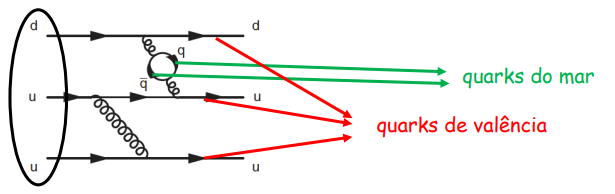
\includegraphics[scale = 0.5]{screenshot/captura20240516011725.png}
    \caption{Composição do proton}
    \label{fig:proton}
\end{figure}
Comumente é utilizado o sabor $q$ para denotar as PDFs , como exemplo
\begin{equation}
    f_u \equiv u(x) = u_v(x) + u_\text{mar}(x) \text{, onde} ~ f_{\bar{u}}(x) = \Bar{u}(x) = u_\text{mar}(x)
\end{equation}
Dessa forma, regra de soma obedece:
\begin{equation}
    \int^\infty_0 (u - \bar{u}) dx =\int^\infty_0 u_v dx= 2
\end{equation}
e
\begin{equation}
    \int^\infty_0 (d - \bar{d}) dx = \int^\infty_0 d_v dx = 1
\end{equation}
Partido da expressão obtida em \eqref{eq:funcaoestruturapdfs} e usando a carga de cada quarks, temos que a função de estrutura para o próton é
\begin{equation}
    \frac{F_2^p}{x} = \frac{1}{9}\qty[4u + d + s + \cdots + 4\bar{u} + \bar{d} + \bar{s} + \cdots ] .
\end{equation}
Usando a simetria de isospin, temos que a função de estrutura de nêutron é
\begin{equation}
    \frac{F_2^n}{x} = \frac{1}{9}\qty[4d + u + s + \cdots + 4\bar{d} + \bar{u} + \bar{s} + \cdots ]
\end{equation}
A partir do teorema óptico, é possível obter que a seção de choque para o foto-absorção  pode ser escrito em termo do tensor hadrônico $W_{\mu\nu}$. De forma que:
\begin{equation}
    \sigma ^{\gamma^* p}_\lambda (x, q^2) = \frac{2\pi^2 \alpha_{em}}{m_p\sqrt{\nu^2 + Q^2}} \varepsilon^{(\lambda)}_\mu \varepsilon_\nu^{(\lambda)*} W^{\mu\nu}
\end{equation}
onde $\varepsilon^{(\lambda)}_\mu$ é o quadrivetor do fóton virtual com helicidade $\lambda$. sabendo que:
\begin{equation}
    \sum_{\lambda=0,\pm 1} \varepsilon^{(\lambda)}_\mu \varepsilon^{(\lambda)*}_\nu  = - \qty(g_{\mu\nu} + \frac{q_{\mu}q_{\nu}}{Q^2}),
\end{equation}
\begin{equation}
    \varepsilon^{(0)}_\mu \varepsilon^{(0)*}_\nu  = - \frac{Q^2}{m_p^2(\nu^2 +Q^2)}\qty(p_{\mu} + \frac{q\cdot p}{Q^2}q_\mu)\qty(p_{\mu} - \frac{q\cdot p}{Q^2}q_\nu)
\end{equation}
e
\begin{equation}
    \frac{1}{2} \qty(\varepsilon^{(+1)}_\mu \varepsilon^{(+1)*}_\nu + \varepsilon^{(-1)}_\mu \varepsilon^{(-1)*}_\nu)  = - \frac{1}{2}\qty(\sum_{\lambda=0,\pm 1} \varepsilon^{(\lambda)}_\mu \varepsilon^{(\lambda)*}_\nu -   \varepsilon^{(0)}_\mu \varepsilon^{(0)*}_\nu)
\end{equation}
obtemos que
\begin{equation}
    \sigma ^{\gamma^* p}_L (x, q^2) = \frac{2\pi^2 \alpha_{em}}{m_p\sqrt{\nu^2 + Q^2}} \varepsilon^{(0)}_\mu \varepsilon_\nu^{(0)*} W^{\mu\nu} = \frac{4\pi^2\alpha_{em}}{Q^2}F_T
\end{equation}
e
\begin{equation}
    \sigma ^{\gamma^* p}_L (x, q^2) = \frac{2\pi^2 \alpha_{em}}{m_p\sqrt{\nu^2 + Q^2}} \frac{1}{2}\qty(\varepsilon^{(+1)}_\mu \varepsilon_\nu^{(+1)*} + \varepsilon^{(-1)}_\mu \varepsilon_\nu^{(-1)*} ) W^{\mu\nu} = \frac{4\pi^2\alpha_{em}}{Q^2}F_L
\end{equation}
onde $F_T$ e $F_L$ são a funções de estrutura transversal e longitudinal, respectivamente.  Além disso, $F_1 = F_T/2x$  e $F_2 = F_L + F_T$. Portanto, a seção de choque total para a foto-absorção pode ser escrita como:
\begin{equation}
    \sigma ^{\gamma^* p} (x, q^2)  =   \sigma ^{\gamma^* p}_L (x, q^2)  +  \sigma ^{\gamma^* p}_T (x, q^2)  = \frac{4\pi ^2\alpha_ {em}}{Q^2}F_ 2(x, Q^2)
\end{equation}
\subsubsection{DGLAP}

\begin{figure}[!ht]
    \centering
    \begin{tikzpicture}
        \begin{feynman}
            \vertex (a);
            \vertex [below right= 1cm and 1cm of a] (b);
            \vertex [below =2.5 cm of a] (c);
            \vertex [below right=1.75cm and 0.5cm of a] (d);
            \vertex [right=1cm  of b] (e);
            \vertex[right = 1cm of d](f);

            \vertex[right = 3cm of a] (g);
            \vertex [below right= 1cm and 1cm of g] (h);
            \vertex [below =2.5 cm of g] (i);
            \vertex [below right=1.75cm and 0.5cm of g] (j);
            \vertex [right=0.7 cm  of h] (k);
            \vertex[right = 2cm of g](l);
            \vertex [right=0.7 cm  of k] (m);

            \vertex[right = 5cm of g] (n);
            \vertex [below right= 1cm and 1cm of n] (o);
            \vertex [below =2.5 cm of n] (p);
            \vertex [below right=1.75cm and 0.5cm of n] (q);
            \vertex [right=0.7 cm  of o] (s);
            \vertex [right=0.7 cm  of s] (u);
            \diagram* {
            (a) -- [boson] (b),
            (c) -- [fermion] (d),
            (d) -- [fermion] (b),
            (b) -- [fermion](e),
            (d) -- [gluon](f),

            (g) -- [boson] (h),
            (i) -- [fermion] (j),
            (j) -- [fermion] (h),
            (h) -- [fermion](k),
            (k) -- [fermion] (m),
            (k) -- [gluon](l),

            (n) -- [boson] (o),
            (p) -- [fermion] (q),
            (q) -- [fermion] (o),
            (o) -- [fermion](u),
            };
            \draw (-0.5,0.1) -- (-0.5,-2.5);
            \draw (6,0.1) -- (6,-2.5);

            \draw (7.5,0.1) -- (7.5,-2.5);
            \draw (13,0.1) -- (13,-2.5);

            \node[right = 0.5cm of e]{$+$};
            \node[right = 4.5 cm of e]{$+$};
            \node[right = 0.5cm of u]{$+ ~~~\text{loops}$};

            \node[above right = 0.8 cm and 4 cm of e]{$2$};
            \node[above right = 0.8 cm and 11 cm of e]{$2$};
        \end{feynman}
    \end{tikzpicture}
    \caption{Diagramas em contribuição em ordem $O(\alpha_s)$ em teoria de pertubação.}
    \label{fig:dglapcorrection}
\end{figure}
O termo obtido na equação \eqref{eq:funcaoestruturapdfs} pode ser tratado como o termo de ordem $0$ da expansão da função de estrutura  $F_2$ como uma série de potência de $\alpha_s$, quando aplicamos teoria de pertubação da QCD. Dessa forma, para adicionarmos correções da QCD e primeira ordem $O(\alpha_s)$, temos que calcular diagramas para os subprocessos apresentados na figura \eqref{fig:dglapcorrection}. O primeiro digrama que aparece no segundo $|\cdots|^2$ é o resultado que conhecemos em \eqref{eq:funcaoestruturapdfs}. Os diagramas identificados como virtual  tratam divergências no ultravioleta. Os diagramas que aparecem no primeiro $|\cdots|^2$ tratam, respectivamente, a possibilidade do párton emitir um glúon antes ou após interagir com o fóton virtual. Re-somando essas contribuições  a função de estrutura, obtemos
\begin{equation}
    \frac{F_2(x,Q^2)}{x} = \sum_q  \int^1_x \frac{dy}{y} f_q(y) e_q^2  \qty[\delta(1-\frac{x}{y}) + \frac{\alpha_s}{2\pi}\qty(P\qty(\frac{x}{y})ln\frac{Q^2}{\mu_0^2} + C\qty(\frac{x}{y}))]
    \label{eq:fedglap}
\end{equation}
onde $P$ e $C$ são funções conhecidas. Aplicando a regra de Feynman para o diagramas apresentados na fig. \eqref{fig:dglapcorrection}  podemos mostrar que
\begin{equation}
    P(z) = \frac{4}{3} \frac{1+z^2}{(1-z)^+} + 2\delta(1-z).
\end{equation}
O termo $ln(Q^2/\mu_0^2)$ que aparece na equação \eqref{eq:fedglap} a partir da integração do espectro do momento transverso do gluon
\begin{equation}
    \int^{Q^2}_{\mu_0^2} \frac{dk_t}{k_t^2} = ln\qty(\frac{Q^2}{\mu_0^2})
\end{equation}
A partir da equação \eqref{eq:fedglap}, podemos redefinir PDFs de forma que tenha dependência da escala $\mu$. As PDFs são redefinidas da seguinte forma:

\begin{equation}
    f_q(x, \mu^2) = f_ q (x) + \int^1_x \frac{dy}{y} f_q(y) \frac{\alpha_s}{2\pi} \qty(P\qty(\frac{x}{y}) ln\qty(\frac{\mu^2 }{\mu_0^2}) + C_1)
    \label{eq:pdfs}
\end{equation}
Dessa forma, a função de estrutura e reescrita da seguinte forma:
\begin{equation}
    \frac{F_2(x,Q^2)}{x} = \sum_q  \int^1_x \frac{dy}{y} f_q(y, \mu^2) e_q^2  \qty[\delta(1-\frac{x}{y}) + \frac{\alpha_s}{2\pi}\qty(P\qty(\frac{x}{y})ln\frac{Q^2}{\mu^2} + C_2)]
    \label{eq:fedglap2}
\end{equation}
Da definição da PDF \eqref{eq:pdfs}, obtemos
\begin{equation}
    \pdv{f_q(x, \mu^2)}{ln\mu^2} = \frac{\alpha_s}{2\pi}\int^1_x \frac{dy}{y} f_q(y, \mu^2) P\qty(\frac{x}{y})
\end{equation}
Esta equação descreve a evolução da PDFs, sendo conhecida na literatura como equação de evolução de DGLAP. Este tratamento em  $O(\alpha_s)$ não está completo. Ao adicionarmos o subprocesso $\gamma q \rightarrow gq$, e preciso que sejam incluídos processos. $\gamma g \rightarrow gq$. Com isso, a equação de evolução DGLAP para PDFs de quarks é reescrita da seguinte forma:
\begin{equation}
    \pdv{q(x, \mu^2)}{ln\mu^2} = \frac{\alpha_s}{2\pi}\int^1_x \frac{dy}{y}\qty(q(y, \mu^2) P_{qq}\qty(\frac{x}{y}) +  g(y, \mu^2) P_{qg}\qty(\frac{x}{y}) )
\end{equation}
onde $g(x,\mu^2)$ é a PDF do glúon e $P_{qg}$ é função de splitting para o proceso  $g\rightarrow q$, dada por:
\begin{equation}
    P_{qg}(z) = \frac{1}{2}(z^2 + (1-z) ^2)
\end{equation}
a PDF do glúon evolue conforme a equação
\begin{equation}
    \pdv{g(x, \mu^2)}{lnQ^2} = \frac{\alpha_s}{2\pi}\int^1_x \frac{dy}{y}\qty(\sum_q(q(y, \mu^2) + \bar{q}(y, \mu^2)) P_{gq}\qty(\frac{x}{y}) +  g(y, \mu^2) P_{gg}\qty(\frac{x}{y}) )
\end{equation}
onde  $P_{gq}$ e $P_{gg}$ são funções de spliting dos subprocessos $q\rightarrow g$ e $g\rightarrow$, respectivamente. É possível mostrar que:
\begin{equation}
    P_{gq} = P_{qq}(1-z) = \frac{1}{4}\frac{1+(1-z)^2}{z}
\end{equation}
e
\begin{equation}
    P_{gg} = 6\qty(\frac{1-z}{z} + \frac{z}{(1-z)_+} + z(1-z)) + \qty(\frac{11}{2} - \frac{n_f}{3})\delta(1-z)
\end{equation}
\begin{figure}
    \centering
    \begin{tikzpicture}
        \begin{feynman}
            \vertex(a);
            \vertex[right = 1cm of a](b);
            \vertex[above right = 0.5 cm and 1cm of b](c);
            \vertex[below right = 0.5 cm and 1cm of b](d);

            \vertex[right = 2.5cm of a](e);
            \vertex[right = 1cm of e](f);
            \vertex[above right = 0.5 cm and 1cm of f](g);
            \vertex[below right = 0.5 cm and 1cm of f](h);

            \vertex[right = 5 cm of a](i);
            \vertex[right = 1cm of i](j);
            \vertex[above right = 0.5 cm and 1cm of j](k);
            \vertex[below right = 0.5 cm and 1cm of j](l);

            \vertex[right = 8 cm of a](m);
            \vertex[right = 1cm of m](n);
            \vertex[above right = 0.5 cm and 1cm of n](o);
            \vertex[below right = 0.5 cm and 1cm of n](p);
            \diagram*{
            (a) -- [fermion](b),
            (b) -- [fermion](c),
            (b) -- [gluon](d),

            (e) -- [fermion](f),
            (f) -- [gluon](g),
            (f) -- [fermion](h),

            (i) -- [gluon](j),
            (j) -- [gluon](k),
            (j) -- [gluon](l),

            (m) -- [gluon](n),
            (n) -- [anti fermion](o),
            (n) -- [fermion](p)
            };
            \node[below = 1cm of a]{$P_{qq}$};
            \node[below = 1cm of e]{$P_{gq}$};
            \node[below = 1cm of i]{$P_{gg}$};
            \node[below = 1cm of m]{$P_{qg}$};
        \end{feynman}
    \end{tikzpicture}
    \caption{Diagramas das funções de spliting }
    \label{fig:spliting}
\end{figure}

Na Fig. \ref{fig:spliting} temos os diagramas  das interações  descritas pelas funções de spliting ($p_{qq}$, $P_{qg}$, $P_{gq}$) em primeira ordem. De maneira geral, $P_{ij}(z)$ representa a probabilidade de um $j$-ésimo párton  irradiar um glúon ou um quarks e se tornar um párton do tipo $i$, com uma fração z do momento do $j$-ésimo párton.

Convenientemente, podemos definir as PDFs  de singleto de sabor ($\Sigma$) e não singleto ($\Delta_q$, já apresentado anteriormente como quark de valência)  como:
\begin{equation}
    \Sigma = \sum_q \qty [q + \bar{q}]
\end{equation}
e
\begin{equation}
    \Delta_q = q - \bar{q} = q_v
\end{equation}

Dessa forma, pode-se mostrar que PDF do quark não singleto obedece à equação de evolução:
\begin{equation}
    \pdv{q}{lnQ^2} = \frac{\alpha_s}{2\pi} \int^1_x \frac{dy}{y} q(y,\mu^2) P_{qq}(\frac{x}{y})
    \label{eq:nosingleto}
\end{equation}
A função não singleto não considera a contribuição dos quarks de mar, e, portanto, dos glúons. Dessa forma, apenas a função $P_{qq}$ aparece em sua evolução.

A equação de evolução da PDF do singleto de sabor pode ser escrita acoplada a equação do glúon da seguinte forma:
\begin{equation}
    \pdv{lnQ^2}\qty(\begin{matrix} \Sigma(x,Q^2) \\g(x,Q^2)\end{matrix}) = \frac{\alpha_s}{2\pi} \int^1_x \frac{dy}{y} \qty(\begin{matrix}
            P_{qq}(\frac{x}{y} ) & P_{qg}(\frac{x}{y}) \\ P_{gq}(\frac{x}{y}) & P_{gg}(\frac{x}{y})
        \end{matrix})\qty(\begin{matrix} \Sigma(x,Q^2) \\g(x,Q^2)\end{matrix})
    \label{eq:singleto}
\end{equation}
As equações  \eqref{eq:nosingleto} e \eqref{eq:singleto} são a forma mais geral de escrever as conhecidas  equações de evolução  Dokshitzer-Gribov-Lipatov-Parisi (DGLAP) . Para pequeno $x$
\subsubsection{BFKL}

A evolução BFKL (Balitsky-Fadin-Kuraev-Lipatov) é uma descrição teórica importante em física de partículas, especialmente no contexto da Cromodinâmica Quântica (QCD). A abordagem BFKL foi desenvolvida para estudar o comportamento das funções de distribuição de partículas em altas energias, particularmente no regime de pequenas frações de momento longitudinal, também conhecido como o regime de \textit{small-x}.

A evolução BFKL visa entender a dinâmica das interações de glúons (as partículas mediadoras da força forte) em altas energias, onde a densidade de glúons é muito alta. Esse regime é crítico para descrever processos de dispersão profunda inelástica e a produção de hádrons em colisões de alta energia, como as que ocorrem no Grande Colisor de Hádrons (LHC).

O parâmetro \(x\) representa a fração do momento longitudinal do hádron carregada pelo glúon. No regime \textit{small-x}, \(x\) é muito pequeno, o que corresponde a altos valores de energia.

A equação BFKL descreve a evolução da densidade de glúons com a energia. É uma equação integral que incorpora a ressumação de diagramas de Feynman de ordem mais alta que se tornam relevantes no regime de pequenas \(x\).

A abordagem BFKL é crucial para entender a produção de quarkonia (estados ligados de quarks pesados) e processos difrativos em altas energias.

A equação BFKL pode ser escrita em uma forma simplificada como uma equação integral para a função de distribuição de glúons \( f(x, k_T^2) \):

\[
    \frac{\partial f(x, k_T^2)}{\partial \ln(1/x)} = \alpha_s K \otimes f(x, k_T^2)
\]

onde:
\begin{itemize}
    \item \(\alpha_s\) é a constante de acoplamento forte.
    \item \(K\) é o núcleo de kernel da equação BFKL, que inclui os efeitos das emissões e absorções de glúons.
    \item \(k_T\) é o momento transverso dos glúons.
\end{itemize}

A evolução BFKL fornece predições para a dependência em energia das seções de choque em processos de dispersão, crucial para experimentos de alta energia.

Considera correções de ordem superior que são negligenciadas em outras abordagens, como a DGLAP (Dokshitzer-Gribov-Lipatov-Altarelli-Parisi).


Resultados da evolução BFKL são comparados com dados experimentais de aceleradores como o HERA e o LHC para verificar a validade da QCD em regimes de alta densidade de glúons.

A equação BFKL é complexa e requer técnicas avançadas de re-sumação e solução numérica.


As correções de próxima ordem (NLO BFKL) introduzem desafios adicionais devido à maior complexidade dos cálculos.



\subsection{GPDs -  Espalhamento Compton Profundamente virtual}
\section{Formalismo de dipolo}
\subsection{Principais descrições - Dglap, BFKL , BK e outros}
\subsection{Modelos fenomenológico - GBW e outros}



\chapter{Produção de mésons vetoriais pesados(HVM)}
\label{cap2}
\section{Formalismo de dipolo (a partir do modelos discutidos no capítulo anterior, apontando a mudança necessária)}
\section{Descrição a partir da GPDs em LO e NLO}

\chapter{Formalismo eiconal} 
\label{cap3}
\section{Aproximação eiconal} 
\section{Colisões fóton-núcleo no formalismo eiconal: Aproximação de Glauber}
\chapter{Aproximação de Weizsäcker-Williams (colisões ultraperiféricas)}
\label{cap4}
\section{O método}
\section{Seções de choque em colisões ultraperiféricas}
\begin{equation}
    F_A(q) = \int d^3\vb{r} e^{i\vb{q}\cdot \vb{r}} \rho_A(r) = \frac{4\pi}{q}\int^{\infty}_0 dr \rho_A(r) r sen(qr)
\end{equation}
\chapter{Fóton-produção exclusiva de mésons vetoriais}
\section{Formalismo de dipolo (com resultados)}
\section{Formalismo de GPDs (com resultados)}

\pagenumbering{arabic}
%\include{pagbranco}
%\include{intro2}
%\include{c5}
\pagenumbering{roman}

\bibliography{biblioteca}


\end{document}
